\documentclass{beamer}
%Information to be included in the title page:
\title{Optimization notes}
\author{Ying-Jia Lin}
\institute{National Cheng Kung University}

\date{May 3rd, 2021}
\setbeamertemplate{footline}[page number]
\begin{document}  
\frame{\titlepage}            
\begin{frame}
    \frametitle{Directional derivative}
    From a starting point $\underline{x}_0$ and a given dirction $\underline{u}$:
    \setbeamertemplate{itemize items}[circle]
    \begin{itemize}
        \item $\underline{x}(\lambda)=\underline{x}_0+\lambda \underline{u}$
        \begin{itemize}
            \item $\lambda$ is a scalar.
        \end{itemize}
        \item \alert{$d\underline{x}=\underline{u}d\lambda$}
        \begin{itemize}
            \item For a small change in $\lambda$.
        \end{itemize}
        \item $F(\lambda)=f(\underline{x}_0+\lambda\underline{u})$
        \begin{flalign*}
            &\begin{aligned}
            dF=df&=(\triangledown f(\underline{x}))^\top d\underline{x}\\
                 &=(\triangledown f(\underline{x}))^\top \alert{\underline{u}d \lambda}
                 =\triangledown ^\top f\underline{u}\lambda
            \end{aligned}&&
        \end{flalign*}
        \item $\frac{df}{d\lambda}=\triangledown ^\top f\underline{u}$
        \begin{itemize}
            \item If $f$ is minimized at $\underline{x}^*=\underline{x}_0+\lambda\underline{u}$, then:
            \begin{itemize}
                \item $\triangledown f(\underline{x}^*))^\top f\underline{u}=0$
                \item gradient $f$ evaluated at the minimum point is orthogonalto $\underline{u}$.
            \end{itemize}
        \end{itemize}
    \end{itemize}
\end{frame}
\begin{frame}
    \frametitle{Weierstrass Theorem}
    If $f(\underline{x})$ is continuous on a nonempty feasible set that is cloased and bounded,
    then $f(\underline{x})$ has a global minimum in this set.
    \begin{itemize}
        \item A set $S$ is bounded if for any point $\underline{x}$ in $S$, we have $\underline{x}^\top \underline{x}<c$
        \begin{itemize}
            \item $c$ is a finite positive number.
        \end{itemize}
    \end{itemize}
    
\end{frame}
\begin{frame}
    \frametitle{Single-variable unconstrained optimization}
    \setbeamertemplate{itemize items}[circle]
    \begin{itemize}
        \item Necessary condition
        \begin{itemize}
            \item If a function $f(x)$ has a local minimum at $x=x^*$,
            and $f'(x)$ exists as a finite number at $x=x^*$, then $f'(x^*)=0.$
            \item $x^*$ at $f'(x^*)=0$ is called stationary point.
        \end{itemize}
        \item Sufficient condition
        \begin{itemize}
            \item Suppose $f'(x^*)=f''(x^*)=\dots =f^{(m-1)}(x^*)=0$,
            but $f^{(m)}(x^*)\neq 0$, then $f(x^*)$ is:
            \begin{itemize}
                \item 1. a local minimum if $f^{(m-1)}(x^*)>0$ and $m$ is even.
                \item 2. a local maximum if $f^{(m-1)}(x^*)<0$ and $m$ is even.
                \item 3. neither a maximum nor a minimum if $m$ is odd.
            \end{itemize}
        \end{itemize}     
    \end{itemize}
\end{frame}

\begin{frame}
    \frametitle{Multi-variable unconstrained optimization (1)}
    Definition of $r^{th}$ differential of function $f$:
    \begin{flalign*}
        &\begin{aligned}
            d^rf(\underline{x}^*)=\sum^n_{i=1}\sum^n_{j=1}\dots\sum^n_{k=1}h_ih_j\dots h_k\frac{\partial^r{f(\underline{x}^*)}}{\partial{x_i}\partial{x_j}\dots\partial{x_k}}
        \end{aligned}&&
    \end{flalign*}
    \textbf{Example}
    
    When (order) $r=2$ and (number of variables) $n=3$, we have:

    \begin{flalign*}
        &\begin{aligned}
            d^2f(\underline{x}^*)&=d^2f(x_1^*, x_2^*, x_3^*)=\sum^3_{i=1}\sum^3_{j=1}h_ih_j\frac{\partial^2f(\underline{x}^*)}{\partial x_i\partial x_j}\\
            &=h^2_1\frac{\partial^2f(\underline{x}^*)}{\partial x^2_1}+
            h^2_2\frac{\partial^2f(\underline{x}^*)}{\partial x^2_2}+
            h^2_3\frac{\partial^2f(\underline{x}^*)}{\partial x^2_3} \\
            &+2h_1h_2\frac{\partial^2f(\underline{x}^*)}{\partial x_1\partial x_2}+
            2h_2h_3\frac{\partial^2f(\underline{x}^*)}{\partial x_2\partial x_3}+
            2h_1h_3\frac{\partial^2f(\underline{x}^*)}{\partial x_1\partial x_3}
        \end{aligned}&&
    \end{flalign*}
\end{frame}


\begin{frame}
    \frametitle{Multi-variable unconstrained optimization (2)}
    \setbeamertemplate{itemize items}[circle]
    \begin{itemize}
        \item Necessary condition
        $$\frac{\partial f(\underline{x}^*)}{\partial x_1}=
            \frac{\partial f(\underline{x}^*)}{\partial x_2}=
            \dots=
            \frac{\partial f(\underline{x}^*)}{\partial x_n}=0$$
        \begin{itemize}
            \item In vector form, $\triangledown f(\underline{x}^*=0)$.
            \item $\underline{x}^*$ at $\triangledown f(\underline{x}^*=0)$ is called stationary point.
        \end{itemize}
        \item Sufficient condition
        \begin{itemize}
            \item For a stationary point at $\underline{x}=\underline{x}^*$:
            \begin{itemize}
                \item if the Hessian matrix of $f(\underline{x})$ evaluated at $\underline{x}=\underline{x}^*$ is \alert{positive definite}, then $\underline{x}^*$ is a local minimum. 
                \item if the Hessian matrix of $f(\underline{x})$ evaluated at $\underline{x}=\underline{x}^*$ is \alert{negative definite}, then $\underline{x}^*$ is a local maximum. 
            \end{itemize}
        \end{itemize}
    \end{itemize}

\end{frame}

\begin{frame}
    \frametitle{Hessian Matrix}
    \setbeamertemplate{itemize items}[circle]
    \begin{itemize}
        \item $(H_f)_{i,j}=\frac{\partial^2f}{\partial x_i \partial x_n}$
        \item In matrix form:     $H_f=\begin{bmatrix}\frac{\partial^2f}{\partial x^2_1} & \frac{\partial^2f}{\partial x_1 \partial x_2}  & \dots & \frac{\partial^2f}{\partial x_1 \partial x_n}\\
            \frac{\partial^2f}{\partial x_2 \partial x_1} & \frac{\partial^2f}{\partial x^2_2}  & \dots & \frac{\partial^2f}{\partial x_2 \partial x_n} \\
            \vdots & \vdots & \ddots & \vdots \\
            \frac{\partial^2f}{\partial x_n \partial x_1} & \frac{\partial^2f}{\partial x_n \partial x_2}  & \dots & \frac{\partial^2f}{\partial x^2_n}
        \end{bmatrix}$
    \end{itemize}
\end{frame}

\begin{frame}
    \frametitle{Definiteness}
    \setbeamertemplate{itemize items}[circle]
    \begin{itemize}
        \item A matrix is positive definite if all its \alert{eigenvalues} are positive.
        \begin{itemize}
            \item If some of the eigenvalues are positive and some are zero, then the matrix is positive semidefinite.
        \end{itemize}
        \item \alert{Checking the sign of the determinants} is an alternative way to determine the definiteness of a matrix.
        \item A twice differentiable function is convex if and only if its Hessian matrix is positive
        semi-definite.
        \begin{itemize}
            \item The function is strictly convex if the Hessian matrix is positive definite.
        \end{itemize}
    \end{itemize}

\end{frame}
\begin{frame}
    \frametitle{Multivariable optimization with equality constraints}
    \textbf{Lagrange Multiplier Theorem}
    \setbeamertemplate{itemize items}[circle]
    \begin{itemize}
        \item Suppose the point $\underline{x}^*$ minimizes $f(\underline{x})$ and satisfies the equality constraints: 
        $h_j(\underline{x}^*)=0$, for $j=1,2,\dots,m$
        \item Assume that the constraint gradients $\triangledown h_j(\underline{x}^*)$ are linealy independent.
        \item Then there exists a unique set $\lambda_j^*$ ($j=1,2,\dots,m$) satisfying:
        $$\frac{\partial L}{\partial x_i}=\frac{\partial f}{\partial x_i}+\sum^m_{j=1}\lambda_j^*\frac{\partial h_j}{\partial x_i}=0$$
        where $i=1,2,\dots,n$.
    \end{itemize}

\end{frame}

\begin{frame}
    \frametitle{Simplex method (Non-linear programming)}
    \textbf{Definition of Simplex}

    The geometric figure formed by a set of n + 1 points in an
    n-dimensional space is called a simplex.

    \setbeamertemplate{itemize items}[circle]
    \begin{itemize}
        \item When the points are equidistant, the simplex is said to be \textit{regular}.
        \item In two dimensions the simplex is a triangle, and in three dimensions, it is a tetrahedron.
        \item The simplex method was originally given by Spendley et al. and was developed later by Nelder and Mead.
    \end{itemize}    
\end{frame}

\begin{frame}
    \frametitle{Simplex method: Steps}
    Choose a reflection coefficient $\alpha>0$, an expansion coefficient $\gamma>1$, and a contraction coefficient $0<\beta<1$.
    \hfill \break
    \begin{enumerate}
        \item Identify $\underline{x}_{\min}$ and $\underline{x}_{\max}$ amoung
            $\{\underline{x}_1, \underline{x}_2,\dots,\underline{x}_{n+1}\}$
            \setbeamertemplate{itemize items}[circle]
            \begin{itemize}
                \item such that $f(\underline{x}_{\min})$ is the minimum
                and $f(\underline{x}_{\max})$ is the maximum
                of all the $f(\underline{x}_i)$, for $i=1, 2, \dots,n+1$.
                \item If $|\underline{x}_{\max}-\underline{x}_{\min}|<\epsilon$, stop.
                The minimum is at $\underline{x}_{\min}$.
                \item Otherwise, let $\underline{x}_a$ be the averaged position of $\{x_1, x_2, \dots, x_{n+1}\}$,
                \textbf{excluding} $\underline{x}_{\max}$, and go to step 2.
            \end{itemize}
        \item Let the reflection point $\underline{x}_r=\underline{x}_a+\alpha (\underline{x}_a-\underline{x}_{\max})$.
        \setbeamertemplate{itemize items}[circle]
        \begin{itemize}
            \item If $f(\underline{x}_{min})>f(\underline{x}_{r})$, let the expansion point $\underline{x}_e=\underline{x}_a+\gamma (\underline{x}_r-\underline{x}_a)$,
            and go to step 3.
            \item Otherwise, go to step 4.
        \end{itemize}
    \end{enumerate}
\end{frame}

\begin{frame}
    \frametitle{Simplex method: Steps}
    \setbeamertemplate{enumerate items}[circle]
    \begin{enumerate}
        \item[3.]If $f(\underline{x}_r)>f(\underline{x}_e)$, the point $\underline{x}_{\max}$ is \alert{replaced} by $\underline{x}_e$.
        \setbeamertemplate{itemize items}[circle]
        \begin{itemize}
            \item Otherwise, $\underline{x}_{\max}$ is \alert{replaced} by $\underline{x}_r$.
            A new set of n+1 points is formed. Then go to step 1.
        \end{itemize}
        \item[4.]If the second largest $f(\underline{x}_i)>f(\underline{x}_{r})$,
         then $\underline{x}_{\max}$ is \alert{replaced} by $\underline{x}_r$ to form a new set of n+1 points,
         and go to step 1.
         \setbeamertemplate{itemize items}[circle]
         \begin{itemize}
             \item Otherwise, go to step 5.
         \end{itemize}
        \item[5.] Let $\underline{x}_p$ be defined such that $f(\underline{x}_p)=\min{\{f(\underline{x}_r), f(\underline{x}_{\max})\}}$
        and let the contraction point $\underline{x}_c=\underline{x}_a+\beta (\underline{x}_p-\underline{x}_a)$.
        \setbeamertemplate{itemize items}[circle]
        \begin{itemize}
            \item If $f(\underline{x}_c)>f(\underline{x}_p)$, \alert{replace} $\underline{x}_j$ by $\underline{x}_j+(\underline{x}_{\min}-\underline{x}_j)/2$, for $j=1,2,\dots,n+1$, and go to step 1.
            \item Otherwise, $\underline{x}_c$ \alert{replaces} $\underline{x}_{\max}$ to form a new set of n+1 points, and go to step 1.
        \end{itemize}
    \end{enumerate}
\end{frame}

\begin{frame}
    \frametitle{Quadratic function}
    $$Q(\textrm{\underline{x}})=\frac{1}{2}\textrm{\underline{x}}^\top\textrm{A}\textrm{\underline{x}}+
    \textrm{B}^\top\textrm{\underline{x}}+\textrm{C}
    $$
    From the two starting points $x_a$ and $x_b$, function minimum is searched along the same direction $\underline{S}$,
    reaching the minimum points $\underline{x}_1$ and $\underline{x}_2$, respectively.
    \begin{figure}
    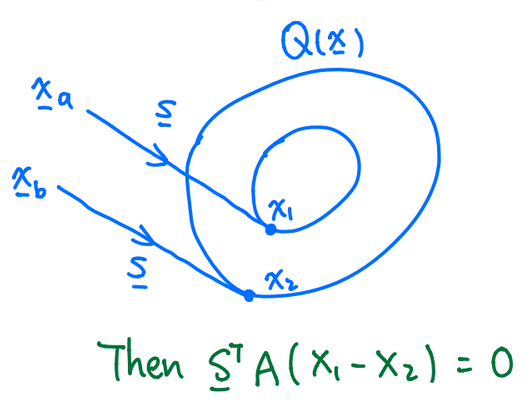
\includegraphics[scale=0.2]{img/quadratic.png}
    \centering
    \end{figure}
    Then the line joining $x_1$ and $x_2$ is $\textrm{A}$-conjugate to $\underline{S}$.
    $\Rightarrow S_i^\top\textrm{A}S_j^\top\neq 0$, for $i\neq j$. $(i=1, 2, \dots,n; j=1,2,\dots,n)$
\end{frame}

\begin{frame}
    \frametitle{Conjugate gradient method}
    During the $(j+1)^{th}$ saerch from point $\underline{x}_{j+1}$, the search direction is given by:
    $$\underline{S}_{j+1}=-\triangledown f(\underline{x}_{j+1})+\beta_j \underline{S}_j$$
    where $$\beta_j=\frac{\triangledown f_{j+1}^\top\triangledown f_{j+1}}{\triangledown f_{j}^\top\triangledown f_{j}}$$
\end{frame}

\begin{frame}
    \frametitle{Conjugate gradient method (Proof - 1)}
    \textbf{From Quadratic function:}
    \begin{align*}f(\textrm{\underline{x}})&=\frac{1}{2}\textrm{\underline{x}}^\top\textrm{A}\textrm{\underline{x}}+
    \textrm{B}^\top\textrm{\underline{x}}+\textrm{C} \\
    f'(\textrm{\underline{x}})&=\textrm{A}\textrm{\underline{x}}+\textrm{B}
    \end{align*}
    \textbf{From steepest descent direction with step length $\lambda$:}
    $$\underline{x}_2=\underline{x}_1+\lambda_1^*\underline{S}_1$$
\end{frame}

\begin{frame}
    \frametitle{Conjugate gradient method (Proof - 2)}
\textbf{Minimize $f$ to obtain the optimized $\lambda^*$:}
\begin{align*}
    \frac{df}{d\lambda_1^*}&=\sum^n_{i=1}\frac{\partial f}{\partial (x_1+\lambda_1^*S_1)}\frac{\partial (x_1+\lambda_1^*S_1)}{\partial \lambda_1^*}\\
    &=\triangledown f(x_1+\lambda_1^*S_1)^\top\cdot S_1 \\
    &=[\textrm{A}(x_1+\lambda_1^*S_1)+\textrm{B}]^\top\cdot S_1 \\
    &=[\alert{\textrm{A}x_1+\textrm{B}}+\textrm{A}\lambda_1^*S_1]^\top\cdot S_1 \\
    &=[\alert{\triangledown f_1}+\textrm{A}\lambda_1^*S_1]^\top\cdot S_1 \\
    &=\triangledown f_1^\top S_1+\lambda_1^*S_1^\top \textrm{A}S_1=0
\end{align*}
Thus, we can get $\lambda_1^*=-\frac{\triangledown f_1^\top S_1}{S_1^\top \textrm{A}S_1}$
\end{frame}

\begin{frame}
    \frametitle{Conjugate gradient method (Proof - 3)}
    \textbf{From steepest descent direction with step length $\lambda$:}
    $$x_2=x_1+\lambda_1^*S_1$$
    $$\Rightarrow \frac{1}{\lambda_1^*}(x_2-x_1)=S_1$$
    Multipliy $\textrm{A}$ and change left and right side:
    $$\Rightarrow \textrm{A}S_1=\frac{1}{\lambda_1^*}\textrm{A}(x_2-x_1)$$
    $$\Rightarrow \alert{S_2^\top\text{A}S_1}=\frac{1}{\lambda_1^*}S_2^\top\textrm{A}(x_2-x_1)=\alert{0}$$
    Currently, we know $\frac{1}{\lambda_1^*}$ is not zero. $\Rightarrow S_2^\top\textrm{A}(x_2-x_1)=0$
\end{frame}

\begin{frame}
    \frametitle{Conjugate gradient method (Proof - 4)}
    \begin{align*}
        S_2^\top\textrm{A}(x_2-x_1)&=S_2^\top(\textrm{A}x_2+\textrm{B}-\textrm{A}x_1-\textrm{B}) \\
        &=S_2^\top(\triangledown f_2 - \triangledown f_1) \\
        &=(-\triangledown f_2+\beta_2S_1)^\top(\triangledown f_2 - \triangledown f_1) \\
        &=-\triangledown f_2^\top\triangledown f_2+\alert{\triangledown f_2^\top\triangledown f_1}-\alert{\beta_2\triangledown f_1^\top\triangledown f_2} + \beta_2\triangledown f_1^\top\triangledown f_1
    \end{align*}
    $\triangledown f_2=\triangledown f_1+\textrm{A}\lambda_1^*S_1
    =\triangledown f_1-\lambda_1^*\textrm{A}\triangledown f_1$ \\
    \begin{flalign*}
        &\begin{aligned}
        \triangledown f_2^\top\triangledown f_1&=(\triangledown f_1-\lambda_1^*\text{A}\triangledown f_1)^\top\triangledown f_1 \\
        &=(\triangledown f_1+\frac{\triangledown f_1^\top S_1}{S_1^\top\textrm{A}S_1}\textrm{A}\triangledown f_1)^\top\triangledown f_1 \\
        &=(\triangledown f_1-\frac{\triangledown f_1^\top \triangledown f_1}{\triangledown f_1^\top\textrm{A}\triangledown f_1}\textrm{A}\triangledown f_1)^\top\triangledown f_1=0\cdot\triangledown f_1=0
        \end{aligned}&&
    \end{flalign*}
\end{frame}

\begin{frame}
    \frametitle{Conjugate gradient method (Proof - 5)}
    Because $\triangledown f_2^\top\triangledown f_1=0$
    \begin{align*}
        \Rightarrow S_2^\top\textrm{A}(x_2-x_1)&=-\triangledown f_2^\top\triangledown f_2+ \beta_2\triangledown f_1^\top\triangledown f_1=0 \\
        \Rightarrow \beta_2&=\frac{\triangledown f_2^\top\triangledown f_2}{\triangledown f_1^\top\triangledown f_1}
    \end{align*}
\end{frame}

\begin{frame}
    \frametitle{Transformation techniques}
    It may be possible to convert a constrained optimization problem into an unconstrained one
    by making a change of variables.
    \hfill \break
    If lower and upper bounds on $x_i$ are specified as:
    $$l_i\leq x_i\leq u_i$$
    which can be satisfied by transforming the variable $x_i$ as:
    $$x_i=l_i+(u_i-l_i)\sin^2y_i$$
    where $y_i$ is the new variable, which can take any value.
    \begin{itemize}
    \item If $x_i$ is restricted to lie in the interval $(0, 1)$, $x_i=\sin^2y$
    \end{itemize}
\end{frame}
\begin{frame}
    \frametitle{Transformation techniques}
    \setbeamertemplate{enumerate items}[circle]
    \begin{enumerate}
        \item The constraints $g_i(\textrm{X})$ must be very simple.
        \item For certain constraints, it may not be possible to find the necessary transformation.
        \item If it is not possible to eliminate all the constraints by making a change of
        variables.
        \setbeamertemplate{itemize items}[circle]
        \begin{itemize}
            \item It may be better not to use the transformation at all.
            \item However, the partial transformation may sometimes produce a distorted objective function which might
            be harder to minimize than the original function.
        \end{itemize}
    \end{enumerate}
\end{frame}

\begin{frame}
    \frametitle{Penalty function method}
    Find $\textrm{X}$ which minimizes $f(\textrm{X})$ is converted into
    an unconstrained minimization problem by constructing a function of the form:
    $$\phi_k=\phi(\textrm{X}, r_k)=f(\textrm{X})+r_k\sum^m_{j-1}G_j[g_j(\textrm{X})]$$
    \setbeamertemplate{itemize items}[circle]
    \begin{itemize}
        \item $g_j$: inequality constraints
        \item $G_j$: some function of the constraint $g_j$
        \item $r_k$: penalty parameter (a positive constant)
        \item $r_k\sum^m_{j-1}G_j[g_j(\textrm{X})]$ is the penalty term.
    \end{itemize}
\end{frame}

\begin{frame}
    \frametitle{Interior and exterior penalty function method}
    \setbeamertemplate{itemize items}[circle]
    \begin{itemize}
        \item Interior method:
        $$G_j=-\frac{1}{g_j(\textrm{X})}$$ or
        $$G_j=-\log[-g_j(\textrm{X})]$$
        \item Exterior method:
        $$G_j=\max[0, g(\textrm{X})]$$ or
        $$G_j=\{\max[0, g(\textrm{X})]\}^2$$
    \end{itemize}
    
\end{frame}

\end{document}